
%(BEGIN_QUESTION)
% Copyright 2006, Tony R. Kuphaldt, released under the Creative Commons Attribution License (v 1.0)
% This means you may do almost anything with this work of mine, so long as you give me proper credit

Anta at vi prøvde å bygge en svært enkel gasskromatograf, der utgangsspenningen fra flammeionisasjonsdetektoren (FID) kobles direkte til en analog skriverskala-registrator:

$$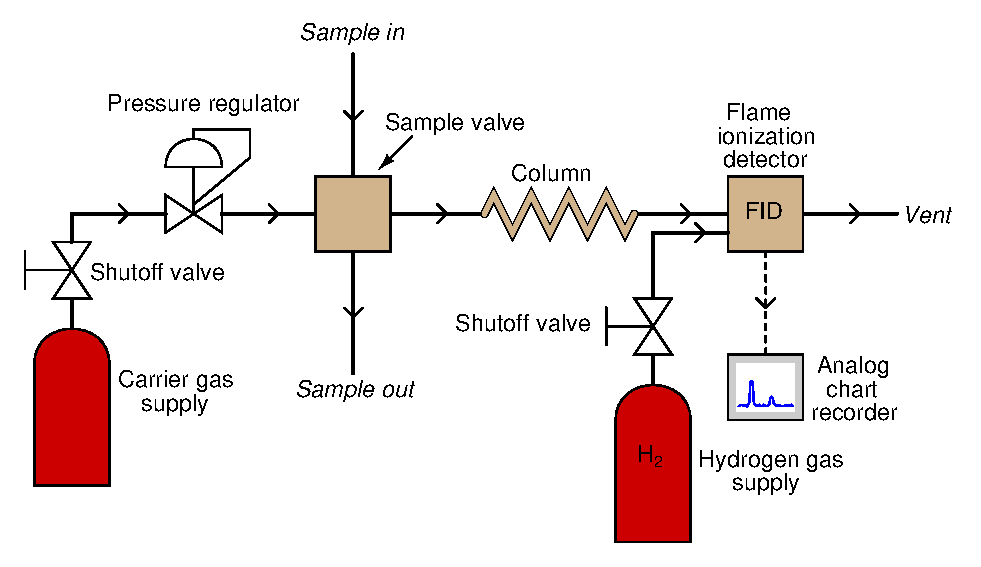
\includegraphics[width=15.5cm]{i01356x01.eps}$$

Denne registratoren vil lage et kromatogram, men det blir et ganske merkelig ett: vi vil ikke kunne tolke det korrekt i rå form. Høyden på toppene i dette kromatogrammet vil {\it ikke} nødvendigvis indikere strømningsratene til de separerte komponentene som kommer ut av kolonnen.

Forklar hvorfor dette kromatogrammet ikke blir korrekt slik det vises, og forklar hva som må til for å korrigere det (dvs. hvordan moderne prosesskromatografer løser dette problemet).

\underbar{file i01356}
%(END_QUESTION)





%(BEGIN_ANSWER)

Problemet er at de ulike forbindelsene som kommer ut av kromatografkolonnen ikke ioniseres like mye i en flamme. Det betyr at topphøydene i kromatogrammet varierer både med komponentens strømningsrate {\it og} med relativ ioniseringsevne.
 
\vskip 10pt

Dette er et grunnleggende problem for alle kromatografer, uansett detektortype. Løsningen er å ``programmere'' forsterkningen til detektoren etter hvilken komponent som forventes å komme ut av kolonnen til et gitt tidspunkt. Dette alene gjør det tydelig hvorfor alle prosesskromatografer er mikroprosessorstyrte.

%(END_ANSWER)





%(BEGIN_NOTES)


%INDEX% Measurement, analytical: chromatography

%(END_NOTES)

